\documentclass[11pt]{article}
\usepackage{graphicx}
\usepackage{amsfonts}
\usepackage{amsmath}
\usepackage{amssymb}
\usepackage{enumitem}
\usepackage{xcolor}

\usepackage[a4paper, margin=1in]{geometry}

\setlength{\headheight}{15pt}
\usepackage{fancyhdr}
\pagestyle{fancy}
\fancyhf{}
\fancyhead[L]{CPSC/EENG 420 - Lab Report 4}
\fancyhead[R]{Bryan SebaRaj  \thepage}

\linespread{1.3} 

\title{Lab 4: Out-of-Order PARCv2 Processor}
\author{Bryan SebaRaj \\[0.5em] Professor Abhishek Bhattacharjee \\[0.5em] EENG 420 - Computer Architecture}
\date{May 7, 2025}

\begin{document}

\maketitle

% Abstract: introductory paragraph summarizing the lab, include a short description of the lab objectives,
% methods, results, and conclusions
% • Design: describe your implementation, justifications for design decisions (if any), deviations from the
% prescribed datapath, discussion of any extensions
% • Testing Methodology: describe how you tested the modules and your overall testing strategy–justify
% the effectiveness of your assembly test(s) in testing the functionality of the processor
% • Evaluation: report your simulation results and cycle counts comparing pv2ooo, pv2spec, and pv2byp
% • Discussion: comparison and analysis of benchmark results in Evaluation, discussion of tradeoffs of
% in-order versus out-of-order (e.g., performance, complexity, workloads, etc.)
% • Figures: updated datapath of the new out-of-order architecture (do not worry about labeling each and
% every wire, focus on the main changes), some diagram of the reorder buffer that was implemented

\subsection*{Abstract}

Out-of-order execution is a technique used in computer architecture design to improve the performance  
a processor by allowing instructions to be executed in a different order than they appear in the program.
This lab focused on implementing an out-of-order PARCv2 processor with a reorder buffer and speculation.
Splitting the implementation into two parts, I first implemented a reorder buffer to allow for out-of-order execution.
I then extended the reorder buffer to support speculation, allowing the processor to 
execute instructions before it is known whether they will be needed.
The processor was tested using a set of benchmarks, including vector add, complex multiply,
masked filter, and binary search. The cycle counts and IPC for each benchmark were recorded and
compared across the two implementations and a baseline pipelined processor with bypassing and no reorder buffer.
The results showed that the out-of-order PARCv2 processors with a reorder buffer and speculation outperformed 
the baseline pipelined processor with bypassing in most cases, demonstrating the benefits of out-of-order execution and speculation.

\subsection*{Design}

\subsubsection*{Objective 1: Out-of-Order PARCv2 Processor with Reorder Buffer}

Given the existing I2O2 PARCv2 processor without a reorder buffer, 
the I2O1 PARCv2 processor was constructed by adding a reorder buffer, 
enabling bypassing out of the reorder buffer in the scoreboard, and
modifying the datapath to enable values to be written from the reorder buffer instead
of from the writeback stage. Specificaly, the reorder buffer was built as a 
16-entry circular queue, with
a four-bit head pointer (commit pointer) and a four-bit tail pointer (allocate
pointer). Each entry comprised a valid bit, a pending bit, and a five-bit field
identifying the destination physical register. 

Allocation is enabled whenever the buffer is not full, which is detected by \texttt{(head\_ptr ==
tail\_ptr) \&\& valid[head\_ptr]}, and, upon handshake, records the incoming
physical register, asserting both valid and pending bits, and advancing the tail
pointer. The fill port handles writeback requests
by deasserting the pending bit of the specified slot, marking that
instruction’s result as ready. Commit logic evaluates \texttt{(valid[head\_ptr] \&\&
!pending[head\_ptr])} each cycle, and if true, deallocates the head entry, issues
the register-file write-enable and corresponding write-address outputs, and
increments the head pointer.

By separating the allocate, fill, and commit pathways and using simple
pointer arithmetic, this should guarantee precise in-order retirement,
support scoreboard‐based bypassing of pending values, and remain 
deadlock-free and readily synthesizable.

\subsubsection*{Objective 2: Out-of-Order PARCv2 Processor with Speculation}

The speculative pv2-spec processor retains the original five-stage PARCv2
datapath but augments its ROB and control logic to allow
instructions to issue and execute past unresolved branches. In my 
implementation, each of the 16 ROB entries has an additional one-bit “speculative” flag
that is set at allocation whenever a branch is present in the Issue stage. All
other fields, valid, pending, and the destination physical register, remain
unchanged. In addition, I added four new control inputs to the ROB: a
speculative-allocation indicator, and three branch-resolution signals
(branch-resolved valid, resolved direction, and mispredict). When a branch
retires in the Execute stage, the ROB scans all entries. On a correct
prediction it simply clears each speculative bit and on a misprediction it
invalidates every speculative entry. 

Note that the commit logic was tightened so that by default only non-speculative, ready
entries retire in-order, preventing speculative results from escaping until
proven correct. By implementing a global invalidate or global
clear approach, rather than precisely tracking the age of each branch, I
minimize additional pointer arithmetic and per-entry state. In the CoreCtrl
module, the original stall-on-branch mechanism was removed so that speculative
instructions flow unimpeded. To address this, branch resolution now drives the ROB’s
speculative bits. Bypass support in the scoreboard and register file was reused
unmodified from Part 1, since speculative and non-speculative values share the
same forwarding paths.

Note that this implementation does not deviate from the prescribed datapath.


\noindent No extensions were implemented.

\subsection*{Testing Methodology}

In order to test correctness, the pipelined processors were tested using the
provided assembly test programs. These were designed to cover all the instructions in MIPS v2 assembly, 
including ALU operations, load and store operations, branch operations, jump operations, 
memory operations. In addition to correctness, performance was also measured with instructions per
cycle and cycle counts through the provided benchmark test suite. 
%
% Two assembly tests were also created to demonstrate that the processor from
% part 2 could simultaneously decode, detect, and handle WAW hazards and simultaneously decode
% two non-ALU instructions. For the former, a simple assembly test was created where two alu operations, specifically 
% \texttt{addiu \$2 1}, where run adjacently. In addition to yielding the correct result, the pipelines were inspected using the \texttt{+disasm=2} flag, 
% to ensure proper WAW hazard detection and stalling (see \texttt{parcv1-wawhaz.S}). For the two non-alu operations, two multiply operations
% were performed adjacently. In addition to yielding the correct result, the pipelines demonstrated simultaneous decoding,
% but stalling before execution (see \texttt{parcv2-2nonalu.S}).

In testing the processor's functionality, I implemented four additional assembly tests that
  verified critical aspects of out-of-order and speculative execution. The
   commit-order-test created a specific dependency chain with a high-latency division operation
  followed by dependent instructions, validating that the ROB correctly maintained program order
  even when execution completes out of sequence. The rob-bypass-test verified the
  processor's ability to bypass values from the ROB that have been written back but not yet
  committed, ensuring instruction-level parallelism doesn't compromise data integrity. 
  The waw-test explores write after write hazards that execute correctly across processor
  implementations due to sufficient time separation, while the better-ipc-test revealed scenarios
  where the simpler bypassing processor achieved better performance than the complex out-of-order and speculative 
  implementations due to ROB management overhead. This comprehensive test suite demonstrated  
  the processors' speculative execution, data forwarding, and commitment mechanisms while targeting
  specific architectural vulnerabilities, providing confidence in the implementations'
  correctness across various dependency patterns. The assembly tests can
  be found in the \texttt{/tests/lab4-custom} directory.


\subsection*{Evaluation}

The pipelined in-order processor with bypassing, pipelined out-of-order processor with the reorder buffer, 
and pipelined out-of-order processor with speculation were tested using the following
benchmarks: vector add, complex multiply, masked filter, and binary search. The
cycle counts and IPC for each benchmark are shown below in the format, cycle
count / IPC.

\begin{center}
    \begin{tabular}{|c || c | c | c|} 
 \hline
 Benchmark & pv2byp & pv2ooo & pv2spec \\
 \hline
 \hline
 binary search & 1749/0.731275 & 1695/0.754572 & 2464/0.519075 \\
 \hline
 complex multiply & 15,312/0.121735 &  2562/0.727557 & 3138/0.594009 \\
 \hline
 masked filter & 13,832/0.32526 & 6248/0.720070 & 7693/0.584817 \\
 \hline
 vector add & 473/0.961945 & 513/0.886940 & 524/0.868321 \\
 \hline

\end{tabular}
\end{center}


\subsection*{Discussion}


Trivial analysis of the performance of the three processors with the provided
benchmarks elucidates the significant benefits of out-of-order execution when
compared to naive, in-order bypassing processor. The simple bypassed in-order
pipeline (pv2byp) delivers excellent performance on straight-line code with
minimal hazards (vector add IPC $\approx$ 0.96) but suffers on high-latency or
data-parallel loops (complex multiply IPC $\approx$ 0.12, masked filter IPC $\approx$ 0.33).
Introducing a 16-entry ROB (pv2ooo) substantially increases instruction‐level
parallelism—raising IPC to 0.73 and 0.72 on those loops. But this is at the expense of
slightly higher cycle time and modest pipeline control overhead, which yields
little or even negative gain on trivial code (vector add IPC drops to 0.89).
Further adding speculative execution (pv2spec) incurs additional misprediction
and commit‐logic overhead. It delivers only marginal benefit over pure
out-of-order on predictable loops and dramatically degrades throughput on
branch-heavy benchmarks (binary search IPC falls from 0.75 to 0.52). Thus,
under the Iron Law (CPU time = IC × CPI × cycle time), the ROB primarily lowers
CPI when ILP is available, speculation can reduce CPI further only if branch
prediction is accurate, and both techniques slightly increase cycle time
without affecting instruction count. As such, their net benefit depends on workload
characteristics.


% This is especially notable in the vector add benchmark, where the IPC of the superscalar processor exceeded 1.
% However, the processor from part 1 of this lab reveals how most of the performance gains of the superscalar processor
% in part 2 are not due to the implemention of two pipelines, but rather the implementation of dual fetch. 
% This is evident in the complex multiply and masked filter benchmarks, where the cycle counts of the dualfetch
% processor was significantly lower than the bypassing processor, and not significantly higher than the IPC
% of the superscalar processor.
%
% Regarding complexity, the implementation of the superscalar processor was significantly more complex than the
% implementation of the bypassing processor and its modification to dualfetch. As such, one could argue that if
% the workload is consistently expected to perform an operation where the dualfetch processor is not significantly slower that the 
% superscalar processor, then one should avoid the additional complexity of the
% superscalar processor construction and instead use the dualfetch processor. Note that these processors follow the Iron Law of 
% Performance, with the most complex processor yielding the best performance, and the simplest processor yielding the worst performance.
% Given that all processors use the same instruction set, the performance gain comes from the reduction in clock cycles / instructions of the 
% more complex processors. 

\subsection*{Figures}

\begin{center}
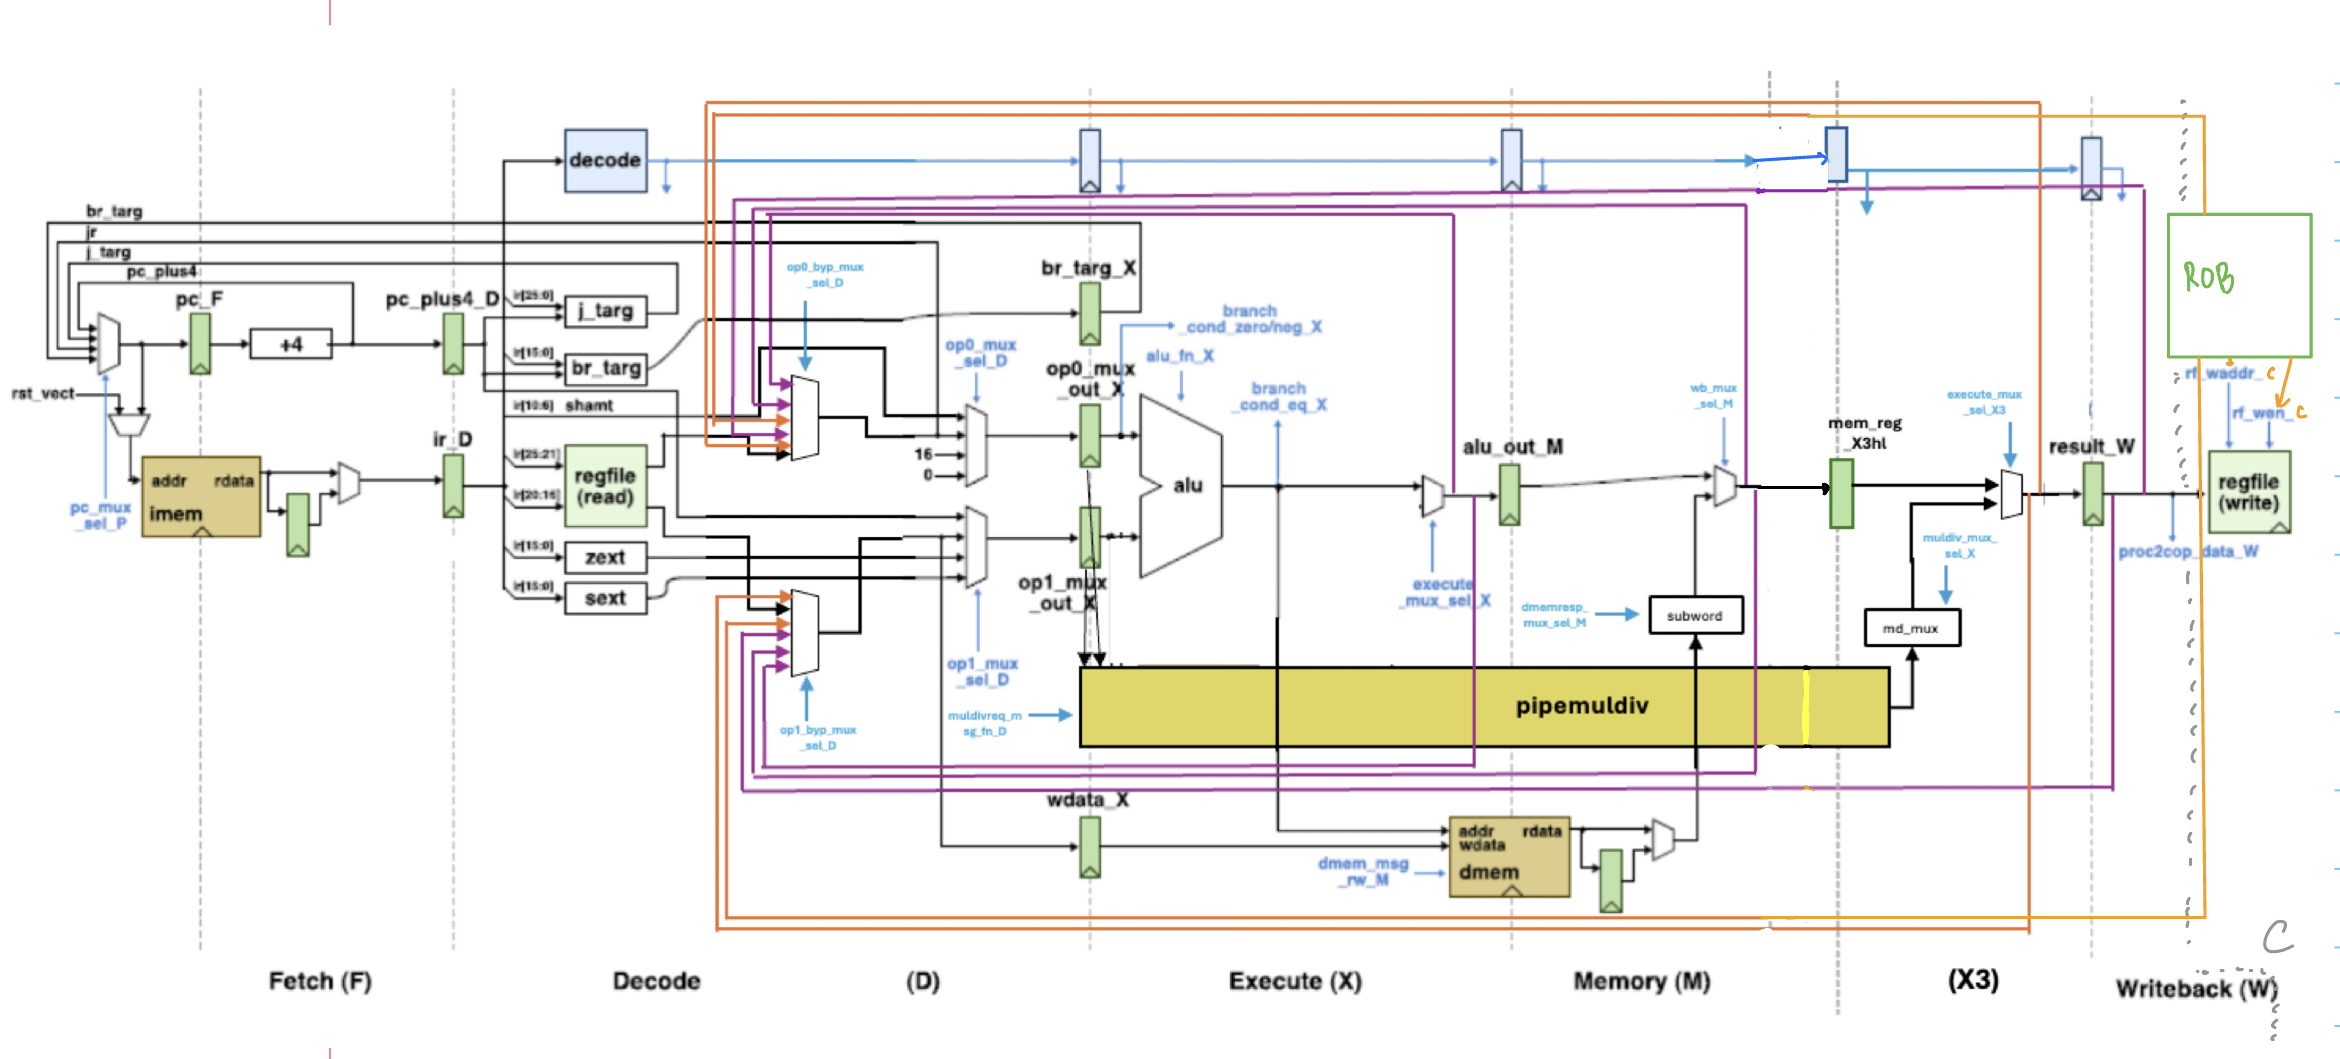
\includegraphics[scale=0.18]{../cpsc420-lab4/pv2ooo-datapath.jpg}
\end{center}
Figure 1. Datapath of out-of-order, single-issue processor.
%See the new muxes within the Decode stage, one for op0 and one for op1. 

\begin{center}
    \begin{tabular}{|p{1in}| p{1in}| p{1.5in} |} 
 \hline
  Valid [6] & Pending [5] & Physical Register [4:0] \\
 \hline
 \hline
  1 & 1 & 4'0011 ($3_{10}$) \\
 \hline

\end{tabular}
\end{center}
Figure 2. Reorder buffer for part 1. Note that the data in the ROB (from the diagram provided on Canvas) live in the pipeline's
writeback stage or go straight to the register file. \\

\begin{center}
    \begin{tabular}{|p{1in}| p{1in}| p{1in} | p{1.5in} |} 

 \hline
 Speculative[7] & Valid [6] & Pending [5] & Physical Register [4:0] \\
 \hline
 \hline
 0 & 1 & 1 & 4'0011 ($3_{10}$)   \\
 \hline

\end{tabular}
\end{center}
Figure 3. Reorder buffer for part 2. Note that the data in the ROB (from the diagram provided on Canvas) live in the pipeline's
writeback stage or go straight to the register file. \\

\begin{center}
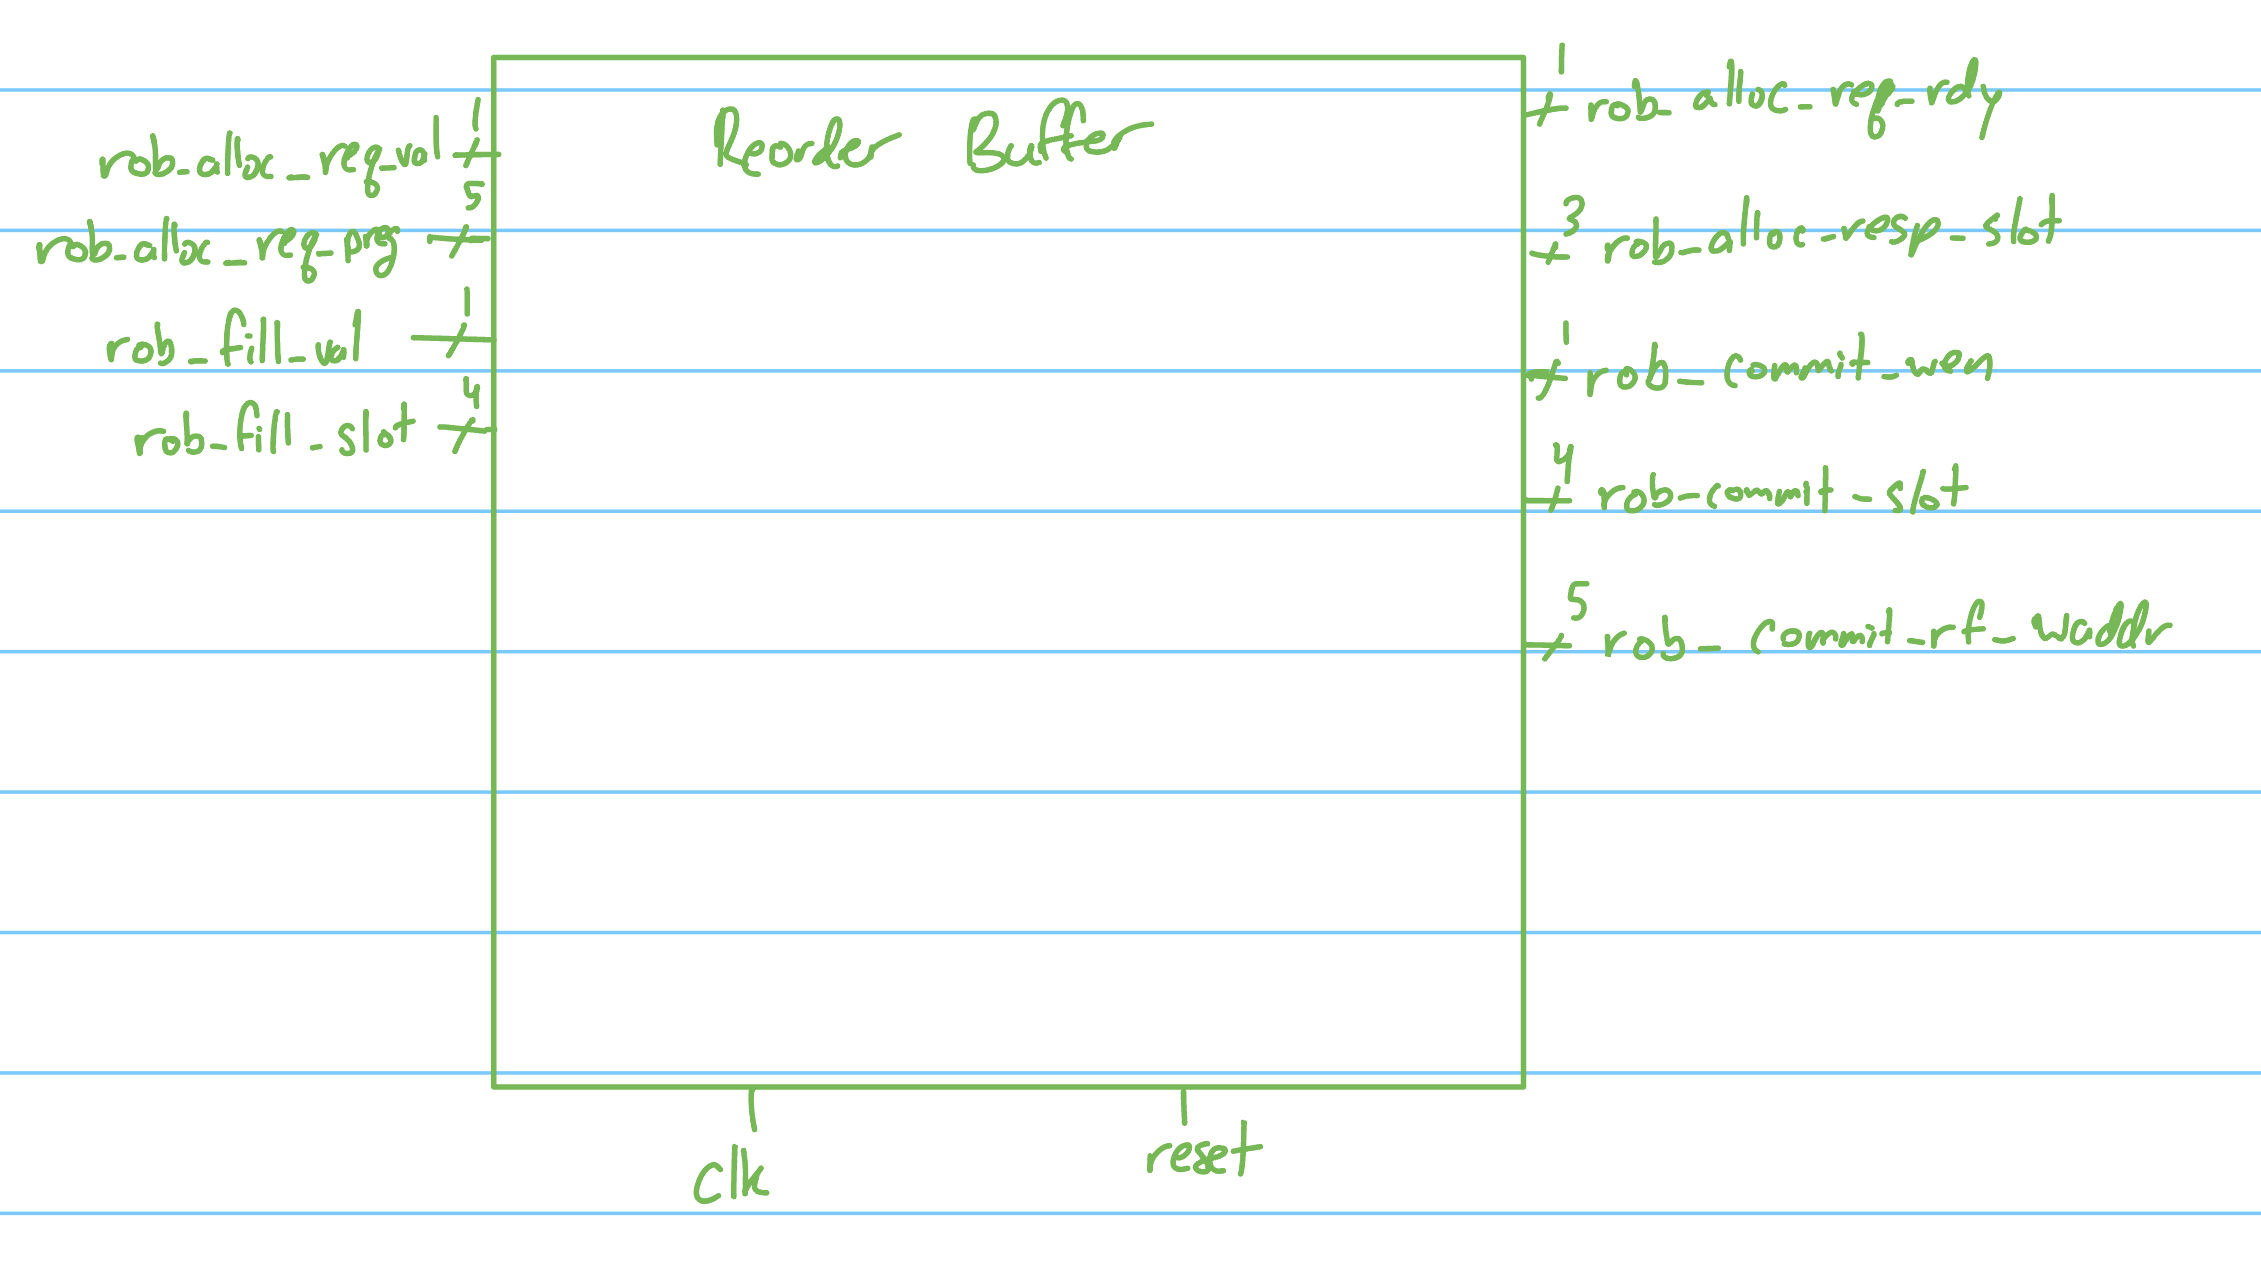
\includegraphics[scale=0.18]{../cpsc420-lab4/pv2ooo-rob.jpg}
\end{center}
Figure 4. Reorder buffer of out-of-order, single-issue processor.

\end{document}


